% Chapter 2

\chapter{Theory and Motivation} % Chapter title

\label{ch:theory} % For referencing the chapter elsewhere, use \autoref{ch:examples} 
This chapter describes the Standard Model of particle physics and its phenomenology in proton-proton collisions at the \ac{LHC}. The shortcomings of the Standard Model are discussed, and Supersymmetry is presented as a possibile solution to many of these shortcomings. Additionally, the simplified Supersymmetric models to be used in the analysis discussed in \autoref{part:search} are introduced. Lastly, Monte Carlo generators, which are used make phenomenological predictions from these models, are described. 

%----------------------------------------------------------------------------------------

\section{The Standard Model}
\label{sec:standard_model}
The \ac{SM} of particle physics describes the interactions of all of the particles currently known to exist, and consists of both matter particles and force carriers. This model has been unprecidentedly successful in predicting new particles and phenomena, including the prediction of the Higgs particle almost 50 years before its discovery in 2012, which completed the \ac{SM}. This section describes the components of the \ac{SM} and how they interact, focusing on the environment of the \ac{LHC}. 

The \ac{SM} is a non-abelian gauge theory blah blah blah

\begin{centering}
\begin{figure}[bth]
\myfloatalign
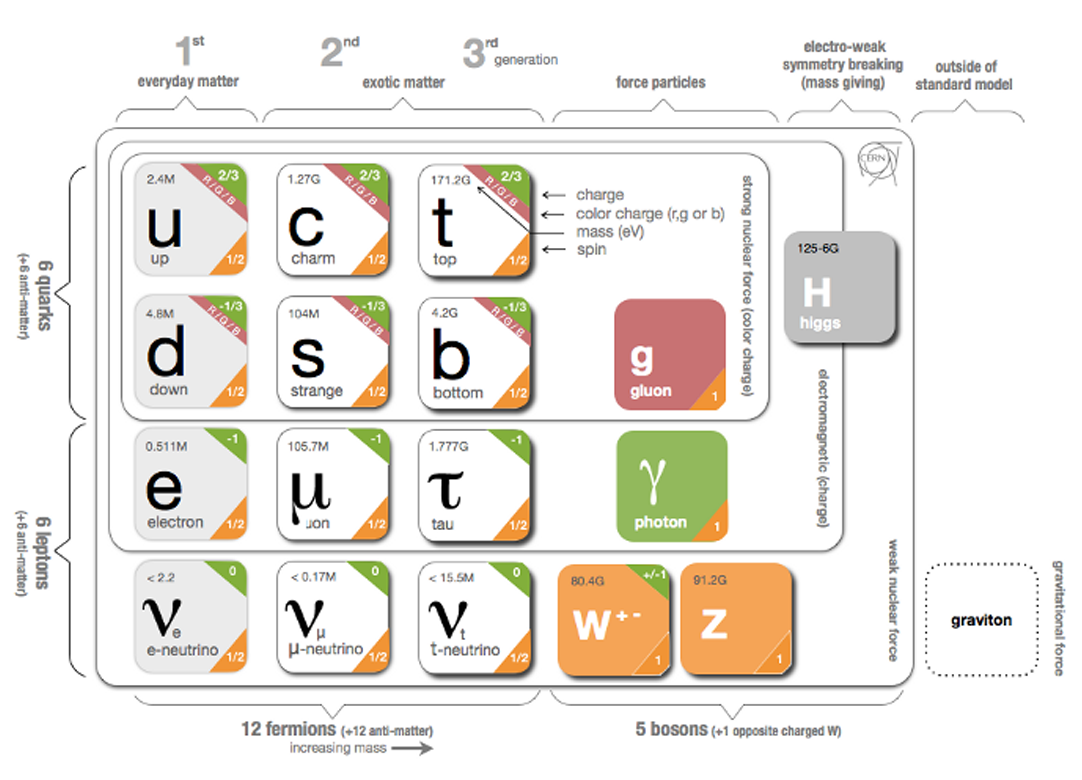
\includegraphics[width=.85\linewidth]{figures/theory/standardmodel.png}
\caption{The Standard Model of particle physics. \cite{Galbraith:2012}}
\label{fig:sm}
\end{figure}
\end{centering}

\subsection{Matter}
The matter described by the \ac{SM} is made up of fermions, spin-$\frac{1}{2}$ particles which can be broken into two groups, quarks and leptons.

\subsubsection{Leptons}


\subsubsection{Quarks}



\subsection{Forces}

\subsection{The Higgs Particle}

\subsection{Phenomenology of Proton-Proton Collisions}
\subsubsection{Parton Distribution Functions}

%------------------------------------------------

\subsection{Problems in the Standard Model}
\label{sec:sm_problems}


%------------------------------------------------

\section{Supersymmetry}

\subsection{Supersymmetry Phenomenology}
\subsection{Solutions to Standard Model Problems}
\subsection{Supersymmetry Signatures in $p-p$ Collisions}
\subsubsection{Simplified Models Used in This Analysis}
\label{sec:simplified_models}

\section{Monte Carlo Generators}
\label{sec:MC_gen}